\section{Результаты}
\subsection{Линейная регрессия}
\subsubsection{Критерий Баумана}
\begin{equation}
\Delta_1(\textbf{X})=
\begin{vmatrix}
1-\varepsilon & 1 \\
1.1-\varepsilon & 1 
\end{vmatrix}
=-0.1
\end{equation}

\begin{equation}
\Delta_2(\textbf{X})=
\begin{vmatrix}
1+\varepsilon & 1 \\
1.1-\varepsilon & 1 
\end{vmatrix}
=-0.1+2\varepsilon
\end{equation}

\begin{equation}
\Delta_3(\textbf{X})=
\begin{vmatrix}
1-\varepsilon & 1 \\
1.1+\varepsilon & 1 
\end{vmatrix}
=-0.1-2\varepsilon
\end{equation}

\begin{equation}
\Delta_4(\textbf{X})=
\begin{vmatrix}
1+\varepsilon & 1 \\
1.1+\varepsilon & 1 
\end{vmatrix}
=-0.1
\end{equation}

Все определители должны иметь отрицательный знак
\begin{equation*}
 \begin{cases}
   -0.1+2\varepsilon < 0\\
   -0.1-2\varepsilon < 0
 \end{cases}
 \Rightarrow 
 \varepsilon<0.05
\end{equation*}

\subsubsection{Признак Румпа}

\begin{equation}
\mathrm{rad}(\textbf{X})=
\begin{pmatrix}
\varepsilon & 0 \\
\varepsilon & 0 
\end{pmatrix}
\quad
\mathrm{mid}(\textbf{X})=
\begin{pmatrix}
1 & 1 \\
1.1 & 1 
\end{pmatrix}
\end{equation}

\begin{equation}
    \sigma(\mathrm{rad}(\mathbf{X}))=\{0,\varepsilon\sqrt{2}\}\Rightarrow\sigma_{\mathrm{max}}(\mathrm{rad}(\mathbf{X}))=\varepsilon\sqrt{2}
\end{equation}

\begin{equation}
\begin{split}
    &\sigma(\mathrm{mid}(\mathbf{X}))=\left\{\sqrt{\frac{421+21\sqrt{401}}{200}},\sqrt{\frac{421-21\sqrt{401}}{200}}\right\}\approx\\
    &\approx\{2.0512, 0.0488\}\Rightarrow\sigma_{\mathrm{min}}(\mathrm{mid}(\mathbf{X}))=0.0488
\end{split}
\end{equation}

\begin{equation}
    \varepsilon\sqrt{2}<0.0488\Rightarrow\varepsilon<0.0345
\end{equation}
\\
\subsubsection{Пример особенной точечной матрицы}
При $\varepsilon=0.05$
\begin{equation}
X=
\begin{pmatrix}
1.05 & 1 \\
1.05 & 1 
\end{pmatrix}
\quad
\mathrm{det}(X)=0
\end{equation}

\subsection{Задачи томографии}
\subsubsection{Критерий Баумана}
\begin{equation}
\Delta_1(\textbf{X})=
\begin{vmatrix}
1-\varepsilon & 1-\varepsilon \\
1.1-\varepsilon & 1-\varepsilon 
\end{vmatrix}
=-0.1+0.1\varepsilon 
\quad
\Delta_2(\textbf{X})=
\begin{vmatrix}
1+\varepsilon & 1-\varepsilon \\
1.1-\varepsilon & 1-\varepsilon 
\end{vmatrix}
=-0.1+2.1\varepsilon-2\varepsilon^2
\end{equation}

\begin{equation}
\Delta_3(\textbf{X})=
\begin{vmatrix}
1-\varepsilon & 1+\varepsilon \\
1.1-\varepsilon & 1-\varepsilon 
\end{vmatrix}
=-0.1-2.1\varepsilon+2\varepsilon^2
\quad
\Delta_4(\textbf{X})=
\begin{vmatrix}
1-\varepsilon & 1-\varepsilon \\
1.1+\varepsilon & 1-\varepsilon 
\end{vmatrix}
=-0.1-1.9\varepsilon+2\varepsilon^2
\end{equation}

\begin{equation}
\Delta_5(\textbf{X})=
\begin{vmatrix}
1-\varepsilon & 1-\varepsilon \\
1.1-\varepsilon & 1+\varepsilon 
\end{vmatrix}
=-0.1+2.1\varepsilon-2\varepsilon^2
\quad
\Delta_6(\textbf{X})=
\begin{vmatrix}
1+\varepsilon & 1+\varepsilon \\
1.1-\varepsilon & 1-\varepsilon 
\end{vmatrix}
=-0.1-0.1\varepsilon
\end{equation}

\begin{equation}
\Delta_7(\textbf{X})=
\begin{vmatrix}
1+\varepsilon & 1-\varepsilon \\
1.1+\varepsilon & 1-\varepsilon 
\end{vmatrix}
=-0.1+0.1\varepsilon
\quad
\Delta_8(\textbf{X})=
\begin{vmatrix}
1+\varepsilon & 1-\varepsilon \\
1.1-\varepsilon & 1+\varepsilon 
\end{vmatrix}
=-0.1+4.1\varepsilon
\end{equation}

\begin{equation}
\Delta_9(\textbf{X})=
\begin{vmatrix}
1-\varepsilon & 1+\varepsilon \\
1.1+\varepsilon & 1-\varepsilon 
\end{vmatrix}
=-0.1-4.1\varepsilon
\quad
\Delta_{10}(\textbf{X})=
\begin{vmatrix}
1-\varepsilon & 1+\varepsilon \\
1.1-\varepsilon & 1+\varepsilon 
\end{vmatrix}
=-0.1-0.1\varepsilon
\end{equation}

\begin{equation}
\Delta_{11}(\textbf{X})=
\begin{vmatrix}
1-\varepsilon & 1-\varepsilon \\
1.1+\varepsilon & 1+\varepsilon 
\end{vmatrix}
=-0.1+0.1\varepsilon
\quad
\Delta_{12}(\textbf{X})=
\begin{vmatrix}
1+\varepsilon & 1+\varepsilon \\
1.1+\varepsilon & 1-\varepsilon 
\end{vmatrix}
=-0.1-2.1\varepsilon-2\varepsilon^2
\end{equation}

\begin{equation}
\Delta_{13}(\textbf{X})=
\begin{vmatrix}
1+\varepsilon & 1+\varepsilon \\
1.1-\varepsilon & 1+\varepsilon 
\end{vmatrix}
=-0.1+1.9\varepsilon+2\varepsilon^2
\quad
\Delta_{14}(\textbf{X})=
\begin{vmatrix}
1+\varepsilon & 1-\varepsilon \\
1.1+\varepsilon & 1+\varepsilon 
\end{vmatrix}
=-0.1+2.1\varepsilon+2\varepsilon^2
\end{equation}

\begin{equation}
\Delta_{15}(\textbf{X})=
\begin{vmatrix}
1-\varepsilon & 1+\varepsilon \\
1.1+\varepsilon & 1+\varepsilon 
\end{vmatrix}
=-0.1-2.1\varepsilon-2\varepsilon^2
\quad
\Delta_{16}(\textbf{X})=
\begin{vmatrix}
1+\varepsilon & 1+\varepsilon \\
1.1+\varepsilon & 1+\varepsilon 
\end{vmatrix}
=-0.1-0.1\varepsilon
\end{equation}\\
Из $\Delta_{6}, \Delta_{10}, \Delta_{15}$ видим, что все определители должны быть отрицательными.\\
Из линейных функций быстрее всех возрастает $\Delta_{8}$, а из квадратичных - $\Delta_{14}$, таким образом
\begin{equation*}
 \begin{cases}
   -0.1+4.1\varepsilon < 0\\
   -0.1+2.1\varepsilon+2\varepsilon^2 < 0
 \end{cases}
 \Rightarrow 
 \varepsilon<\frac{1}{41}
\end{equation*}

\subsubsection{Признак Румпа}
\begin{equation}
    \mathrm{rad}(\mathbf{A})=\begin{pmatrix}
    \varepsilon&\varepsilon\\
    \varepsilon&\varepsilon
    \end{pmatrix}\quad
    \mathrm{mid}(\mathbf{A})=\begin{pmatrix}
    1&1\\
    1.1&1
    \end{pmatrix}\quad
\end{equation}
\begin{equation}
    \sigma(\mathrm{rad}(\mathbf{A}))=\{0,2\varepsilon\}\Rightarrow\sigma_{\mathrm{max}}(\mathrm{rad}(\mathbf{A}))=2\varepsilon
\end{equation}
\begin{equation}
\begin{split}
    &\sigma(\mathrm{mid}(\mathbf{X}))=\left\{\sqrt{\frac{421+21\sqrt{401}}{200}},\sqrt{\frac{421-21\sqrt{401}}{200}}\right\}\approx\\
    &\approx\{2.0512, 0.0488\}\Rightarrow\sigma_{\mathrm{min}}(\mathrm{mid}(\mathbf{X}))=0.0488
\end{split}
\end{equation}
\begin{equation}
    2\varepsilon<0.0488\Rightarrow\varepsilon<0.0244
\end{equation}
\subsubsection{Пример особенной точечной матрицы}
При $\varepsilon=\frac{1}{41}$
\begin{equation}
A=
\begin{pmatrix}
1+\frac{1}{41} & 1-\frac{1}{41} \\
1.1 - \frac{1}{41}& 1+\frac{1}{41} 
\end{pmatrix}
\quad
\mathrm{det}(A)=0
\end{equation}

\subsection{Глобальная оптимизация}
\textbf{Функция МакКормика.}\\
\begin{figure}[H]
\centering
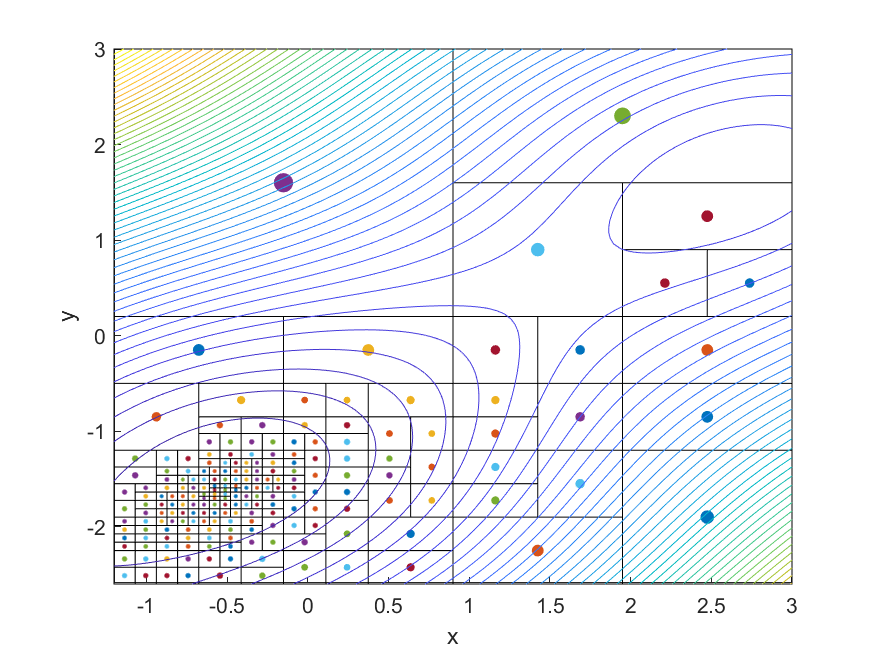
\includegraphics[width=0.85\textwidth]{Graphics/McCormick_algo.png}
\caption{Положения брусов и их центров для функции МакКормика \eqref{McCormick}} 
\end{figure}
\begin{figure}[H]
\centering
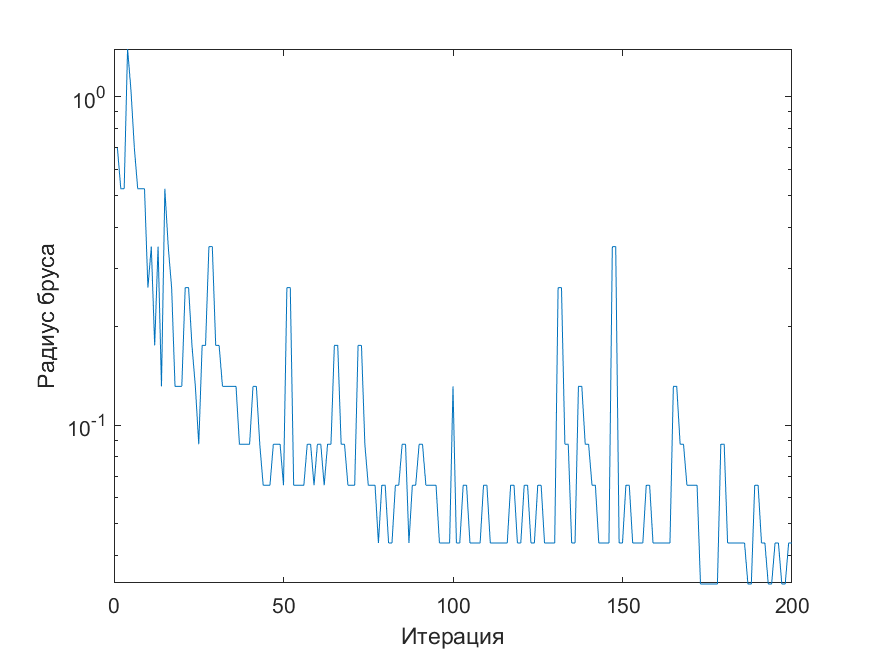
\includegraphics[width=0.85\textwidth]{Graphics/McCormick_bar_rad.png}
\caption{Радиусы брусов для функции МакКормика \eqref{McCormick}} 
\end{figure}
\begin{figure}[H]
\centering
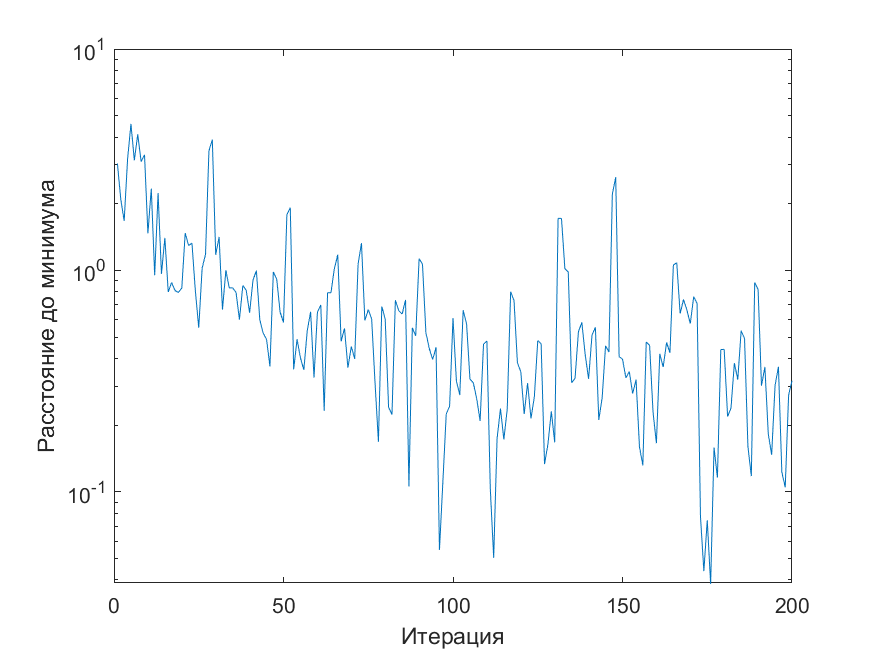
\includegraphics[width=0.85\textwidth]{Graphics/McCormick_dist_to_min.png}
\caption{Расстояние до точки минимума для функции МакКормика \eqref{McCormick}} 
\end{figure}
\noindent\textbf{Функция Химмельблау.}\\
\begin{figure}[H]
\centering
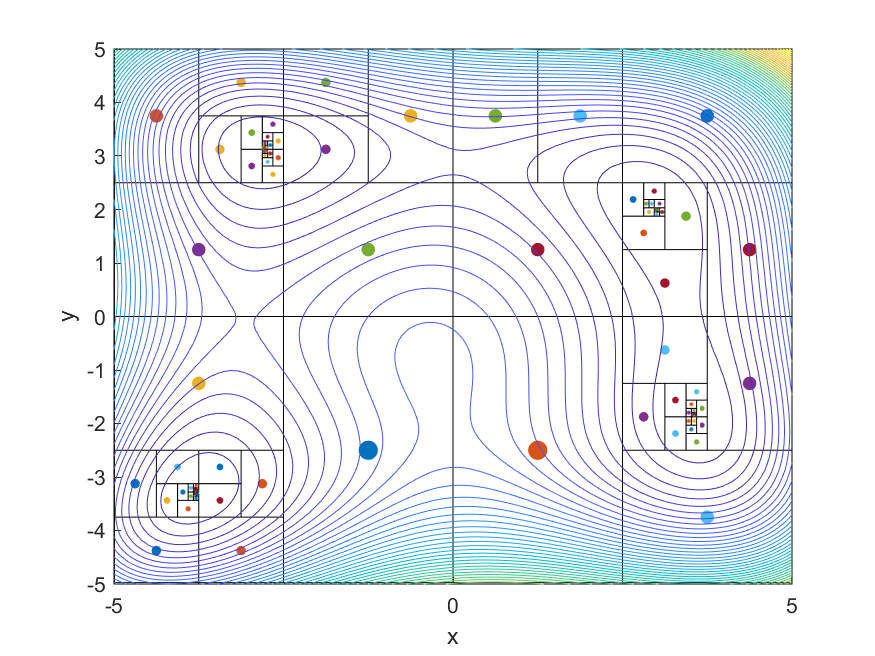
\includegraphics[width=0.85\textwidth]{Graphics/Himmelblau_algo.png}
\caption{Положения брусов и их центров для функции Химмельблау \eqref{Himmelblau}} 
\end{figure}
\begin{figure}[H]
\centering
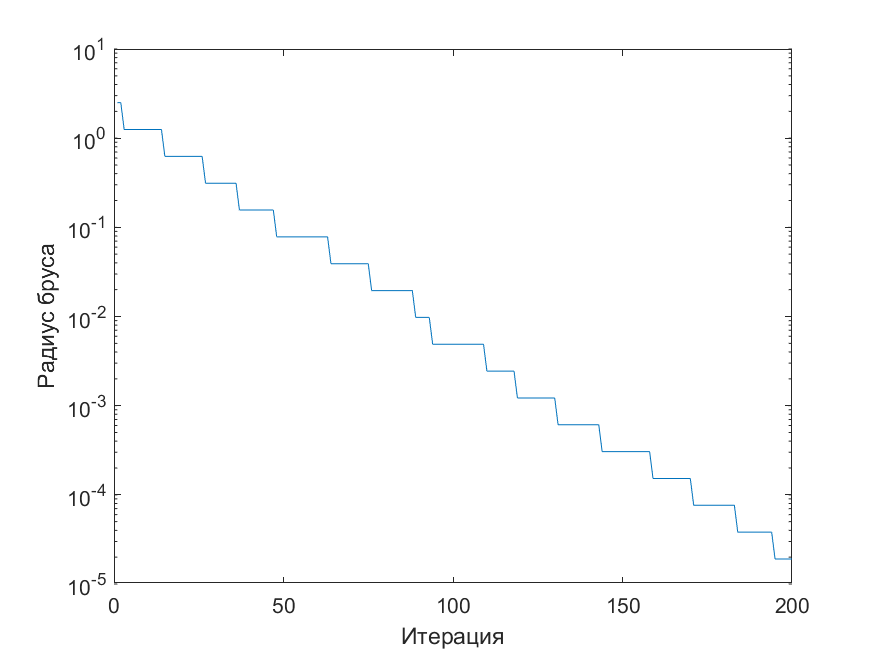
\includegraphics[width=0.85\textwidth]{Graphics/Himmelblau_bar_rad.png}
\caption{Радиусы брусов для функции Химмельблау \eqref{Himmelblau}} 
\end{figure}
\begin{figure}[H]
\centering
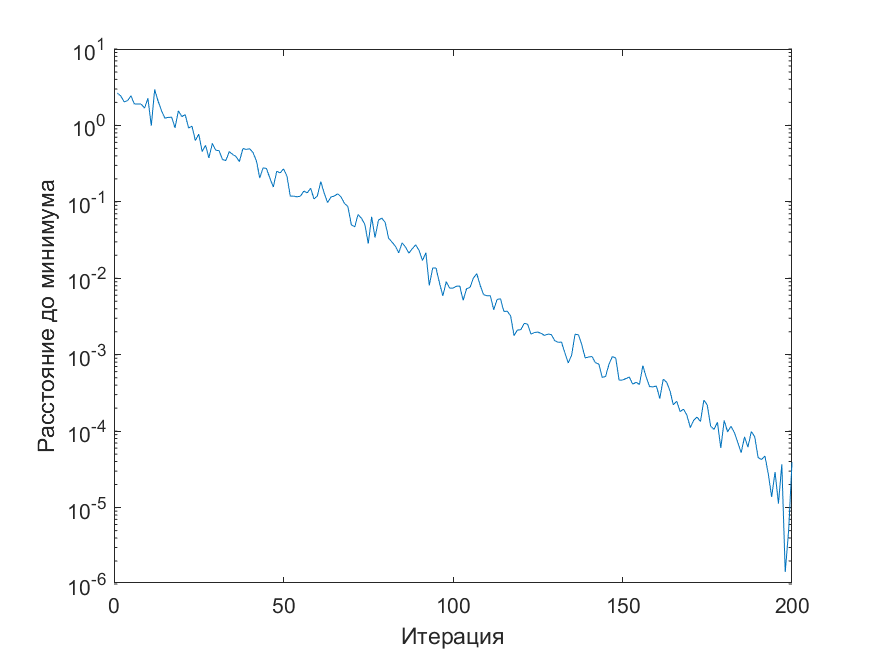
\includegraphics[width=0.85\textwidth]{Graphics/Himmelblau_dist_to_min.png}
\caption{Расстояние до точки минимума для функции Химмельблау \eqref{Himmelblau}} 
\end{figure}